\documentclass{article}


% if you need to pass options to natbib, use, e.g.:
%     \PassOptionsToPackage{numbers, compress}{natbib}
% before loading neurips_2024


% ready for submission
\usepackage{neurips_2024}


% to compile a preprint version, e.g., for submission to arXiv, add add the
% [preprint] option:
%     \usepackage[preprint]{neurips_2024}


% to compile a camera-ready version, add the [final] option, e.g.:
%     \usepackage[final]{neurips_2024}


% to avoid loading the natbib package, add option nonatbib:
%    \usepackage[nonatbib]{neurips_2024}

\usepackage{graphicx} 
\usepackage[utf8]{inputenc} % allow utf-8 input
\usepackage[T1]{fontenc}    % use 8-bit T1 fonts
\usepackage{hyperref}       % hyperlinks
\usepackage{url}            % simple URL typesetting
\usepackage{booktabs}       % professional-quality tables
\usepackage{amsfonts}       % blackboard math symbols
\usepackage{nicefrac}       % compact symbols for 1/2, etc.
\usepackage{microtype}      % microtypography
\usepackage{xcolor}         % colors

\usepackage{biblatex} %Imports biblatex package
\addbibresource{bibliography.bib} %Import the bibliography file

\title{Semiconductor Layout Design with Large Language Models: Opportunities and Challenges}

\author{%
  Bo Wen\\
  IBM Watson Research Center, \\
  Yorktown Heights, NY, USA \\
  \texttt{bwen@us.ibm.com} \\
  \And
  Xin Zhang\\
  IBM Watson Research Center, \\
  Yorktown Heights, NY, USA \\
  \texttt{xzhang@us.ibm.com} \\
}

\begin{document}

\maketitle

\begin{abstract}
  This paper explores the potential of large language models (LLMs) as a ``layout design copilot'' in semiconductor and integrated circuit (IC) design. We evaluate the baseline performance of state-of-the-art LLMs on a set of 25 layout design tasks, revealing common mistakes and limitations. We explores spatial reasoning and knowledge application capabilities of LLMs through the Via Connection test case. We introduce a novel Neuro-inspired LLM Reasoning Network architecture, called SOLOMON, which significantly improves performance on these tasks. The paper discusses the challenges of using LLMs in layout design and brainstorms future research directions.
\end{abstract}

\section{Introduction}
The semiconductor industry faces significant challenges in automating the layout design for integrated circuits (ICs), microfluidic chips, and other electronic devices. Current graphical user interface (GUI) based design workflows lack adaptability, leading to inefficient, repetitive tasks when creating similar structures with minor variations.\cite{Greengard2024-hx} This approach violates the ``Don't Repeat Yourself'' (DRY) principle and reduces productivity.

While traditional layout design software has struggled to address these challenges, Large Language Models (LLMs) offer a promising solution. LLMs' ability to understand natural language instructions and generate code makes them ideal candidates for a ``layout design copilot''. This new paradigm could allow human designers to focus on high-level tasks requiring creativity and intuition, while the LLM-powered copilot generates or modifies the layout code based on human intent.

This paper explores the capabilities and limitations of LLMs in semiconductor layout design tasks. We evaluate the baseline performance of state-of-the-art LLMs, document an iterative design process with multimodal inputs, and introduce a novel Neuro-inspired LLM Reasoning Network architecture to improve reasoning capabilities and mitigate hallucinations.

\section{Baseline LLM Performance in Layout Design}

We evaluated the performance of five large language models (LLMs) - GPT-4o\cite{GPT-4o}, Claude-3.5-Sonnet\cite{Claude-3.5-Sonnet}, Llama-3.1-70B\cite{Llama-3.1-70B}, Llama-3.1-405B\cite{Llama-3.1-405B} and the new ``reasoning model'', o1-preview\cite{o1-preview} - on a set of 25 layout design tasks. Each tasks have been run 5 times with same prompt and temperature = 0.7. The LLMs are asked to write a python code with gdspy\cite{gdspy} and generate a GDSII file. We then run the LLM written code in a Linux VM and further convert the generated GDSII file to png images for human evaluation. These tasks were categorized into four groups: Basic Shapes 1, Basic Shapes 2, Advanced Shapes, and Complex Structures. Figure \ref{fig:baseline-llm-performance} presents a summary of the LLMs' performance across the task categories. See Appendix for the task prompts and detailed results.

\begin{figure}[h]
  \centering
  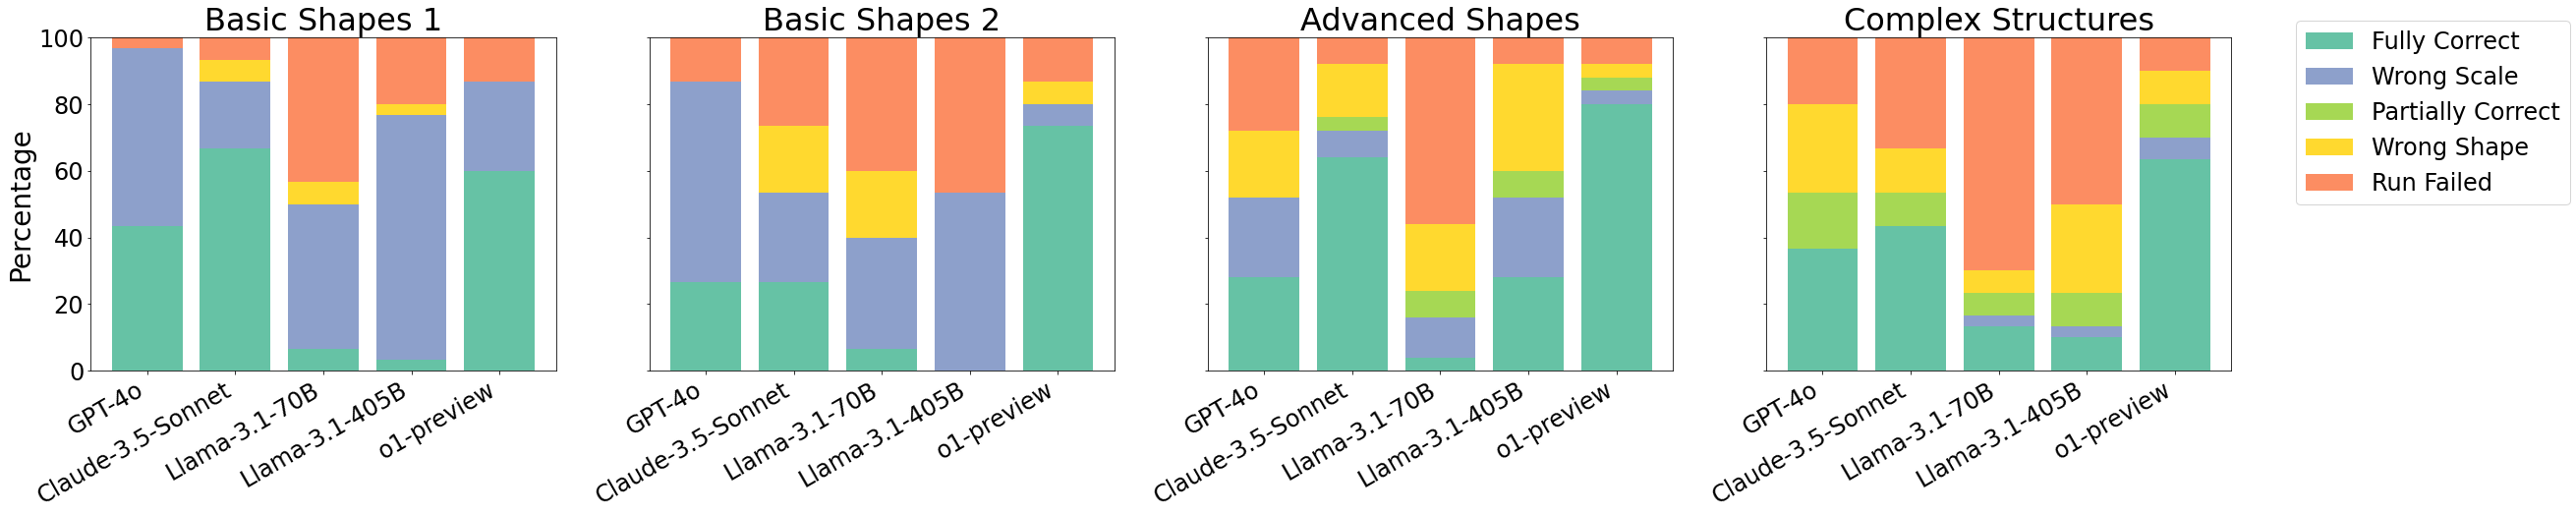
\includegraphics[width=\textwidth]{baseline-llm-performance.png}
  \caption{Baseline LLM Performance on Layout Design Tasks}
  \label{fig:baseline-llm-performance}
\end{figure}

The results reveal several common mistakes and limitations of standalone LLMs in handling layout design tasks:

  1. \textbf{Incorrect scaling}: The default unit in the gdspy library is micrometers. But we requested the basic shapes to be drawn in millimeters, in order to test whether the LLM could correctly figure out this catch and scale the shapes according to the specified units. As can be seen from the dark blue ``Wrong Scale'' part of bar chart, all the LLMs struggled to various degrees: (a) Sometimes the LLMs simply failed to pay attention to the requested unit (millimeters) and did not perform the necessary scaling. (b) In some cases, LLMs did pay attention to the requested unit but made incorrect assumptions about gdspy's default unit. We observed many hallucinations of millimeters (Llama) and a few cases of nanometers (Claude) or meters (GPT-4o). Especially when multiple units are mentioned in the prompt, LLMs are more likely to hallucinate. (c) From the chart, we can see that Llama-3 models are especially vulnerable to this issue. They sometimes even assumed the user had made a mistake by requesting millimeters, and proceeded to draw in micrometers instead, justifying this choice with comments like "not mm, as the GDSII format is in micrometers". This type of ``arrogant'' behavior and misalignment with human instructions on simple tasks will be very harmful for deploying LLMs as fully automanous AI agents. A recent Nature paper \cite{ZhouNature2024} has also discussed similar observations.
  
  2. \textbf{Partial correctness}: In more complex tasks, LLMs sometimes generated partially correct result with right shapes but wrong relative positions. This is shown in the light green ``Partially Correct'' part of the bar chart.
  
  3. \textbf{Wrong shapes}: Incorrect shapes often result from LLMs making basic arithmetic errors. For instance, in the ``Hexagon'' task, Llama-3.1-405B once used an internal angle of 120 degrees, producing a triangle instead of a hexagon. However, in other runs, it correctly calculated the angle based on the number of edges. Many of these errors can be mitigated through Chain-of-Thought (CoT) prompting, which encourages the model to do calculations step-by-step.

  4. \textbf{Runtime errors}: Approximately one third of the generated code from the evaluated LLMs resulted in exceptions and failed to execute. The most frequent error, \textit{AttributeError: module 'gdspy' has no attribute 'LayoutViewer'}, occurred 26 times (59.09\%) with GPT-4o and 33 times (61.11\%) with Claude-3.5-Sonnet. In contrast, this error was reported only once each for Llama-3.1-70B and o1-preview, and not at all for Llama-3.1-405B, indicating that GPT-4o and Claude-3.5-Sonnet are trying to be ``helpful'' by providing GUI output (sometimes this is provided in comments), which is not available in the runtime environment and caused errors. This is not entirely LLM's fault, but due to missing specification about runtime environment in the prompt. In order to make a fair comparison, we re-ran the generated code with `LayoutViewer' line commented out. Figure \ref{fig:baseline-llm-performance} are showing the adjusted results. The second most common errors were due to hallucinations of nonexistent `gdspy` functions or methods, including various `AttributeErrors` (e.g., `'CrossSection'`, `'Circular'`, `'Ellipse'`) and `TypeErrors`. This also includes spelling error, for example, miss spelling \textit{gdspy.Text} as \textit{gdspy.text}. Additionally, other frequent issues involved typical programming logic mistakes such as missing module imports or incorrect function parameters. For more details, see the error report in (Appendix).
  
  5. \textbf{Inefficient code}: There's one special case that we'd like to point out. In the DLDChip task, which involves creating a dense array of identical shapes, the Llama-3.1-405B model generated a code that created a large number of objects and performed numerous boolean operations, leading to high memory usage and extended execution time. We have to kill the code after about 15 mins of waiting. 

  6. \textbf{Ambiguous instructions}: In some of the results, we observed that the LLMs results mainly fall into two categories. After inspecting the prompts, we found that the instructions can be interpreted in two ways. In this case, we count both type of results as correct. But when implementing copilot, the agent should ask for clarification if the instructions are ambiguous.

Many of these issues can be mitigated by augmenting the LLMs with more advanced setup. Specifically, using Retrieval-Augmented Generation (RAG) to provide gdspy documentation to the LLMs, we should be able to reduce the errors related to misspelling and hallucinating nonexistent functions. For complex tasks, we can provide example code of simple shapes for In-Context Learning, so the LLMs only need to reason about positioning and scaling, and avoid runtime errors. We will discuss more in Section 3.

\section{Multimodal Inputs and Spatial Reasoning}
Layout design in semiconductor processes requires not only generating correct basic geometric shapes but also spatial reasoning to create proper ``layouts'' that meet specific requirements. Via connections, which create electrical pathways between different chip layers, exemplify this challenge. While seemingly simple—typically consisting of circular vias and rectangular metal connections—they demand precise positioning and sizing to ensure no short or open circuits and other functionality issues.

We conducted a series of tests by providing a sketch(image) together with different text prompts. The sketch are color-coded to represent different layers (e.g., yellow for via, blue for metal, red for pad) to help LLM understand the spatial relationships. We varied the text prompts to test the LLMs' spatial reasoning. We used GPT-4o's vision input capability for this experiment. Figure \ref{fig:via_experiment} illustrates the sketch inputs and corresponding LLM-generated outputs for each test case.

\begin{figure}[!h]
\centering
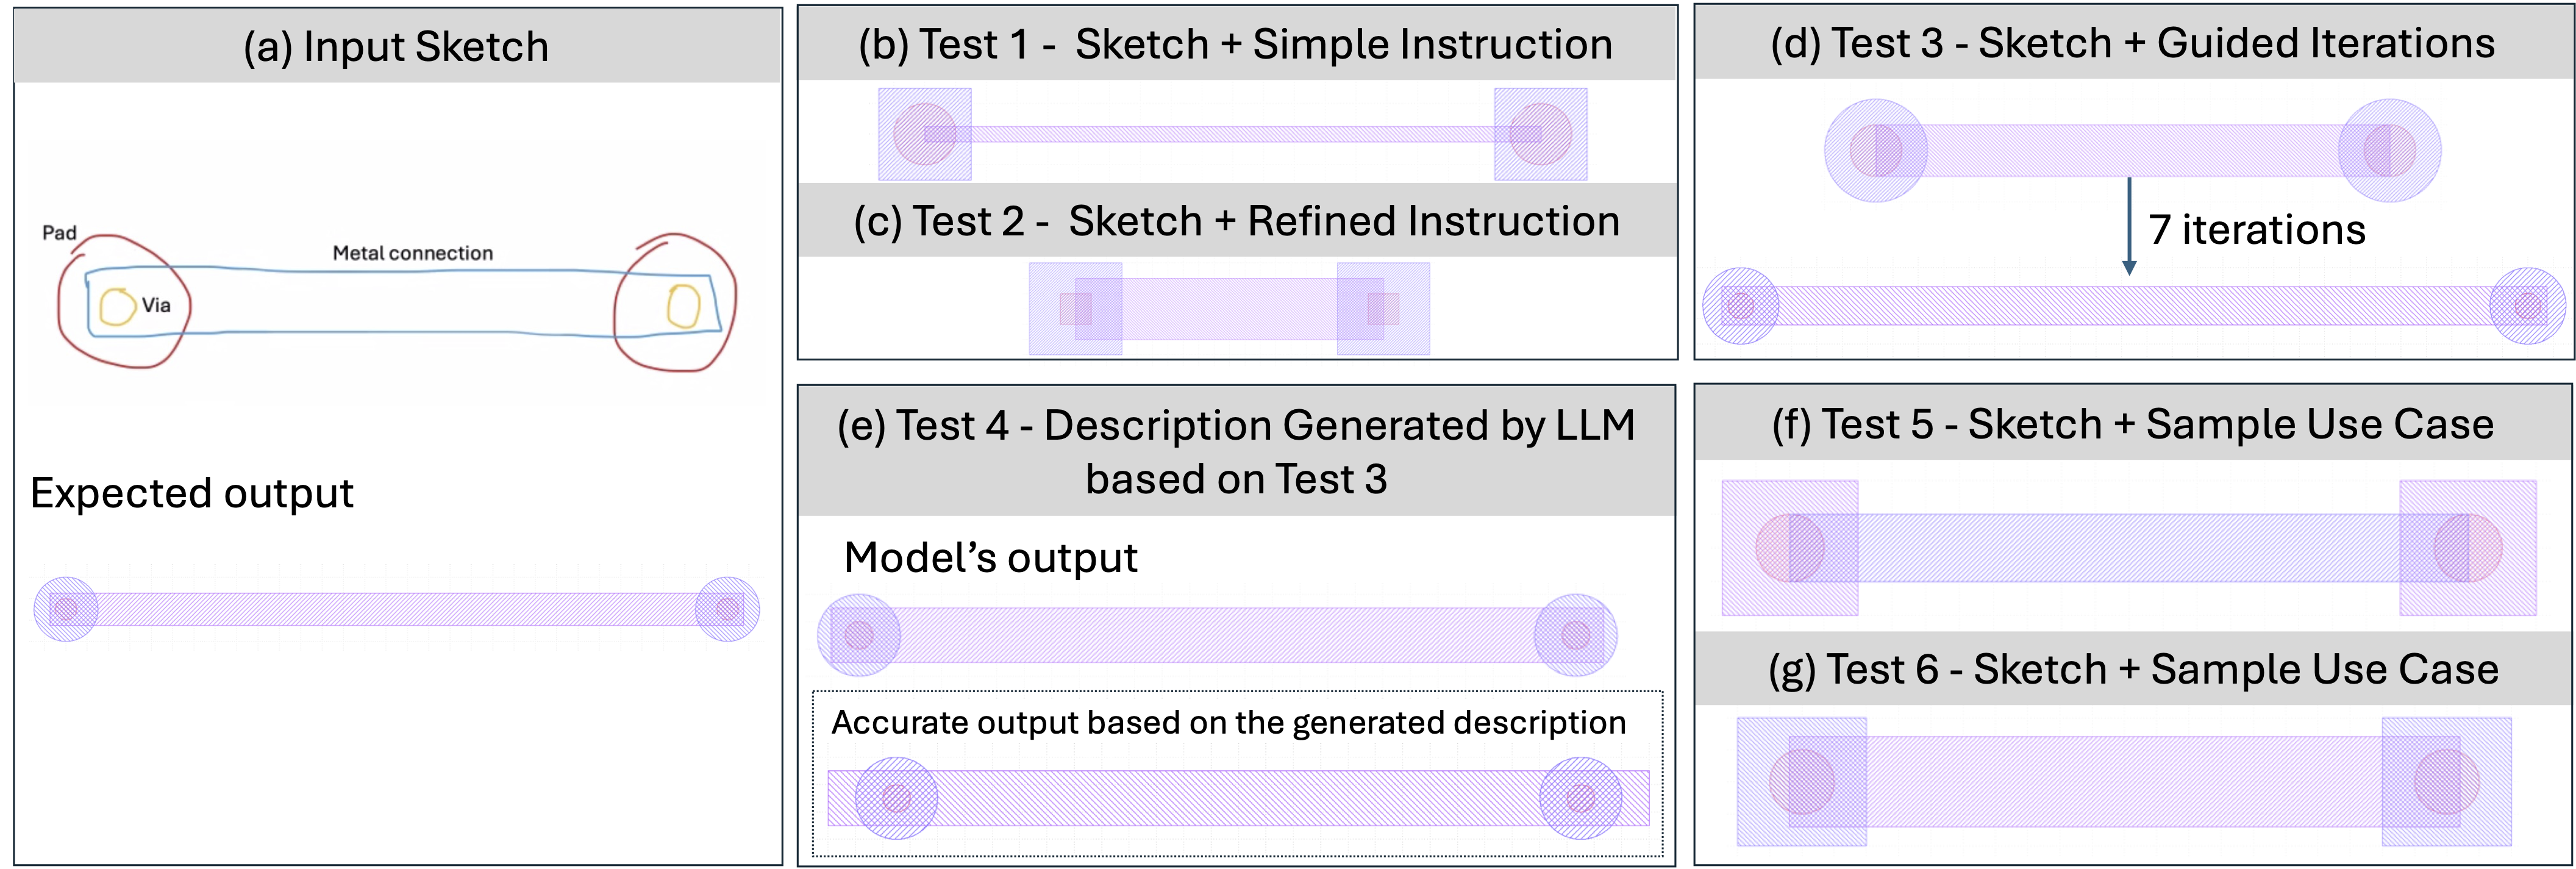
\includegraphics[width=1\linewidth]{Figure1_v5.png}
\caption{Sketch input and LLM-generated outputs for the via connection experiment. The sketch depicts a desired layout with two vias connected by a metal layer and circular pads on top. The outputs show the progression of the LLM's understanding and refinement of the layout based on iterative feedback and context provided by the user.}
\label{fig:via_experiment}
\end{figure}
In \textbf{Test 1}, we provided a basic sketch (Figure ~\ref{fig:via_experiment}(a)) with simple instructions. The LLM generated code, but the output had issues, including insufficient metal connection width. \textbf{Test 2} involved refining the description, but the output incorrectly used square vias and pads, and failed to properly cover the vias with metal. In \textbf{Test 3}, we provided a more detailed description. The initial output still had issues like not fully covering the vias with the metal connection, and the metal width was equal to the via's radius. So we engaged in an iterative prompting conversation, providing the LLM with feedback and screenshots of the GDSII file generated from its code. After seven iterations, the LLM finally produced the correct layout (Figure ~\ref{fig:via_experiment}(d)).

\textbf{Test 4} reversed the process by asking the LLM to create a detailed prompt based on the correct layout from \textbf{Test 3} (Appendix). The LLM described each component's size and location in detail but hallucinated an additional requirement: \textit{a 50-unit space between the vias and the edges of the metal connection}. This would result in the layout shown in the dotted rectangle in Figure~\ref{fig:via_experiment}(e), where the metal extends beyond the contact pad. Interestingly, when given this ``wrong'' prompt, GPT-4o ignored the added specification and produced a layout matching the original design, with the metal not extending beyond the pad. Code inspection revealed that the LLM used another requirement, \textit{Leave a margin of 10 units between the edge of the metal and the pads}, to calculate the metal edge position in both x and y directions, although this was intended only for the y-direction margin. Using this version of prompt in the baseline evaluations (Section 1), o1-preview and Llama-3.1-405B each produced the ``non-extending'' version in one out of 5 runs, indicating some ambiguity in the specification. Generally, providing specific numerical values for size and location of geometric shapes in the prompt proves more robust than simple instructions like ``draw me a via''.

To further test our hypothesis, we conducted \textbf{Tests 5} and \textbf{6}, removing numerical values from the prompt and incorporating domain-specific context (e.g., 3D packaging and Through-Silicon Vias). This approach, however, degraded LLM performance, revealing a critical limitation: while LLMs possess textbook knowledge of semiconductor concepts, they struggle to translate this into practical design requirements. For instance, LLMs failed to apply common engineering knowledge, such as using wider metal layers to connect vias or leaving margin space between components in different layers to account for layermisalignment.

This finding underscores the importance of improving LLMs' reasoning capability of applying domain knowledge in problem-solving, rather than simply increasing model size to remember more knowledge, to enhance the adaptability of LLM-based AI systems.

\section{Neuro-inspired LLM Reasoning Network Architecture}

Based on the observations from the previous sections, we hypothesize that LLMs' poor performance in layout design tasks is due to their weak reasoning ability in spatial tasks, as well as their poor performance in applying domain knowledge. 

To test this hypothesis, we run the 25 tasks through the IBM properitary System for Optimizing Language Outputs through Multi-agent Oversight Networks (SOLOMON). SOLOMON is designed as part of a grant proposal in response to the ARPA-H ADVANCED RESEARCH PROJECTS AGENCY FOR HEALTH CHATBOT ACCURACY AND RELIABILITY EVALUATION (CARE) EXPLORATION TOPIC. It is designed to detect and correct LLM hallucinations in healthcare applications. It is based on a Neuro-inspired LLM Reasoning Network Architecture inspired by the Brain-like AGI \cite{Brain-AGI} and the Free Energy Principle (FEP) theory \cite{FEP}. Due to page limit and compliance restrictions, we will not go into the details of the architecture here. We plan to publish the architecture in near future. On high level, the key idea is to combine multiple LLMs with different knowledge bases (trained on different data) and reasoning abilities (instruction following and alignment fine-tuning) to form a pool of Thought Generators, and then use another LLMs based Thought Assessor system, which leverages Free Energy Principle to analyze the consensus and differences from the ensemble of proposed ``Thoughts'', then generate a final output based on the instruction from a Steering Subsystem, which in the current version is a human.

\begin{figure}[h]
  \centering
  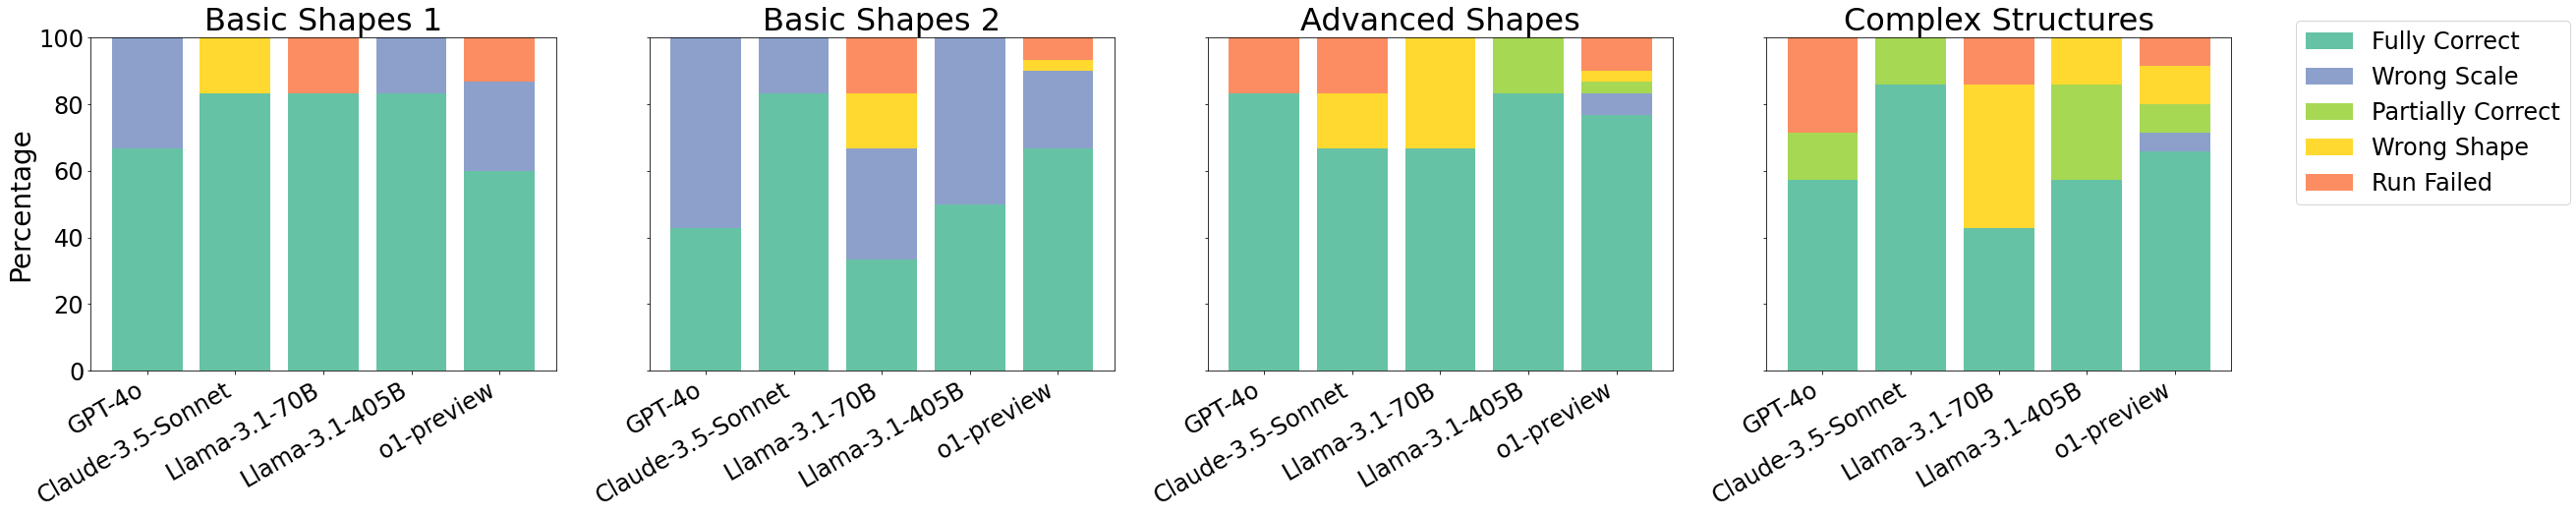
\includegraphics[width=\textwidth]{judges-performance.png}
  \caption{Performance comparison between 4 instances of SOLOMON built with classic non-reasoning LLMs versus o1-preview, the SOTA of reasoning LLM.}
  \label{fig:judges-performance}
\end{figure}

Figure \ref{fig:judges-performance} shows the SOLOMON' performance on same 25 tasks. We used the 5 runs from GPT-4o, Claude, and 2 Llama-3.1 models, total 20 ``Thoughts'', including the code, error report, and rendered GDSII images (but only for GPT-4o and Claude, because the Llama-3.1 models doesn't support vision input); and then we created 4 instances of SOLOMON each using one of the 4 LLMs acting as a Thought Assessor to assess the 20 ``Thoughts'' in order to generate an improved results. The o1-preview result in the figure is copied from the baseline LLM performance, only showing for comparison purpose. We can see that performance is improved for all the 4 LLMs compared to their baseline, especially the runtime error is almost completely eliminated. It is also noticible that the improvement for GPT-4o and Claude are more significant than for Llama-3.1 models, which is due to the fact that they can provide vision input which assists the spatial reasoning. Without the vision input, the Llama-3.1 models can only avoid the runtime errors, but cannot evaluate which ``Thought'' is better in terms of spatial layout.

\section{Conclusion and Future Work}
The introduction of the SOLOMON architecture significantly improved performance, particularly in reducing runtime errors and enhancing spatial reasoning capabilities. However, challenges remain in translating domain knowledge into practical design requirements.

Future research directions include:
1. Creating comprehensive benchmarks for LLM capabilities in layout design tasks.
2. Exploring more configurations of SOLOMON architecture to understand the interaction between quality of initial thoughts vs assessment by ensemble, i.e., system 1 vs system 2 contributions in reasoning tasks.
3. Exploring stacking layers of SOLOMON architecture to form a hierarchical reasoning model, for recalling and reasoning domain knowledge for solving the task on hand.
4. Exploring the adaptability of SOLOMON architecture across different domains.

While LLMs show promise as layout design copilots, further advancements in reasoning capabilities and domain knowledge application are necessary for their effective integration into semiconductor design processes and other domain specific tasks.

\textbf{Acknowledgment:} We thank Kuan Yu Hsieh for her valuable contribution in creating the dataset of 25 tasks with ground truth and her exploration work on the via connection test cases.

\printbibliography %Prints bibliography

\newpage
\appendix

\section{Appendix / supplemental material}
\subsection{Prompt Used in Via Connection Test Cases}
\textbf{Prompt for Test 1:}
"I have a sketch idea that i want to draw in GDSII, generate the python code for this design. each color represents an individual layer. We want to use a metal to connect two vias and put a pad on top of each via"; with graphical input of the sketch:
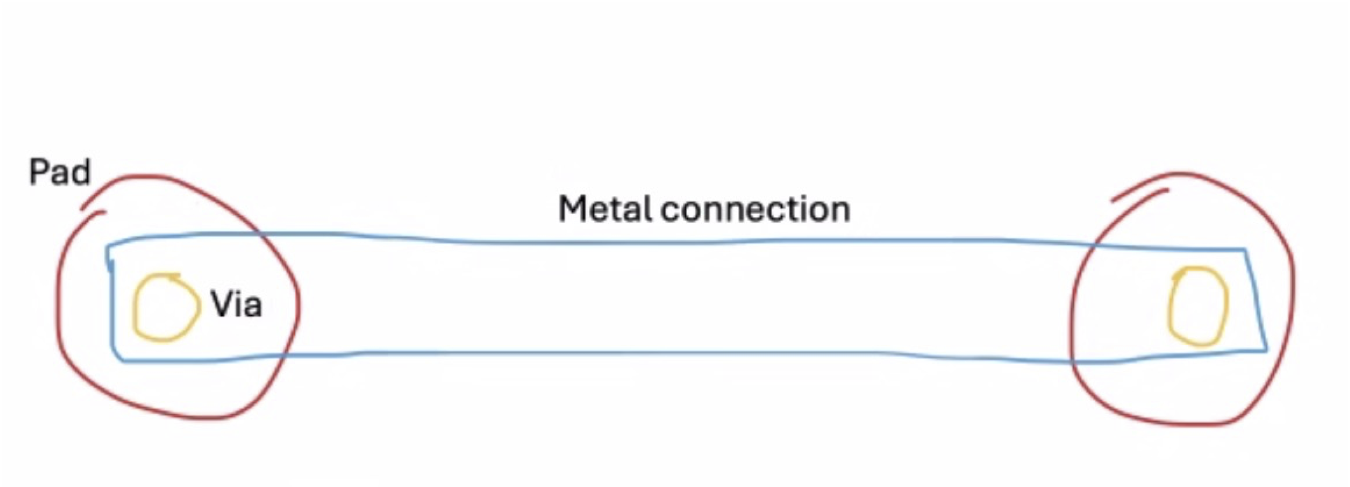
\includegraphics[width=0.5\linewidth]{sketch.png}

\textbf{Prompt for Test 2:} "I have a sketch idea that i want to draw in GDSII, generate the python code for this design. each color represents an individual layer. We want to have two vias near each end on a piece of metal. And a pad on top of the metal."; with graphical input of the sketch:
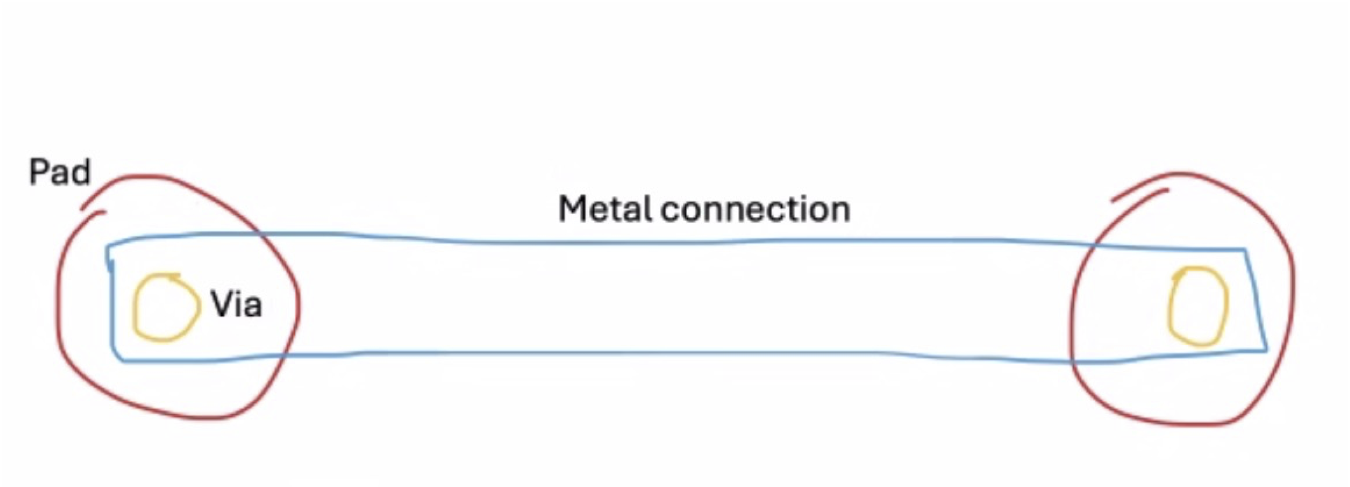
\includegraphics[width=0.5\linewidth]{sketch.png}

\textbf{Prompt for Test 3:} "I have a sketch idea that i want to draw in GDSII, generate the python code for this design. each color represents an individual layer. we want use to connect two vias using a piece of metal and put a circular padding on top of each via"; with graphical input of the sketch:
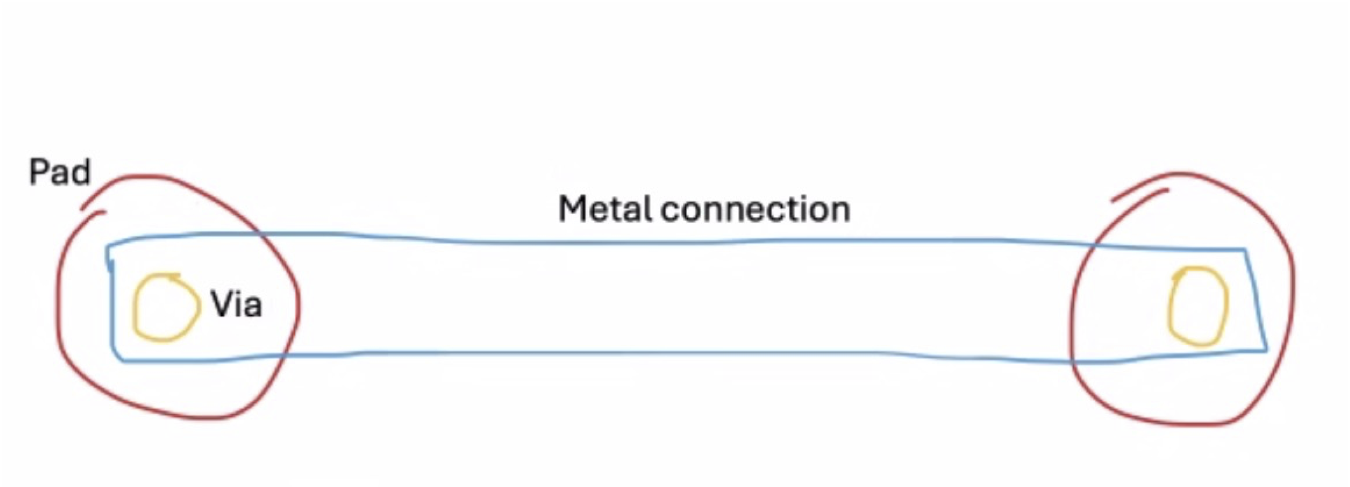
\includegraphics[width=0.5\linewidth]{sketch.png}

\textbf{Prompt for Test 4 (Generated by LLM based on the final output in Test 3):}\\
"Layers and Colors:
The design consists of three layers: via layer (yellow), metal layer (blue), and pad layer (red).\\
Dimensions:
Via: The radius of each via is 10 units.
Pad: The radius of each pad is 30 units.
Metal Connection: The width of the metal connection is 40 units, and the total length is 600 units.\\
Positions:
The first via is positioned at coordinates (50, 150).
The second via is positioned at coordinates (550, 150).\\
Connections and Coverage:
The metal connection should fully cover the vias, extending slightly beyond their edges.
Ensure the metal connection is slightly wider than the via diameter to provide full coverage.\\
Spacing and Margins:
Leave a margin of 10 units between the edge of the metal and the pads.
Ensure there is a space of 50 units between the vias and the edges of the metal connection.\\
Additional Requirements:
The metal connection should be shorter than the total length to fit beneath the covering area of the pads, leaving some space at the edges.
By providing detailed information like this, you can ensure that the design is accurately reproduced. If you have any specific design rules or preferences, make sure to include those as well."

\textbf{Prompt for Test 5:}"I have sketched a design for 3d packaging, where we have a metal connecting two TSVs , please generate the python code to draw a GDSII for this design."; with graphical input of the sketch: 

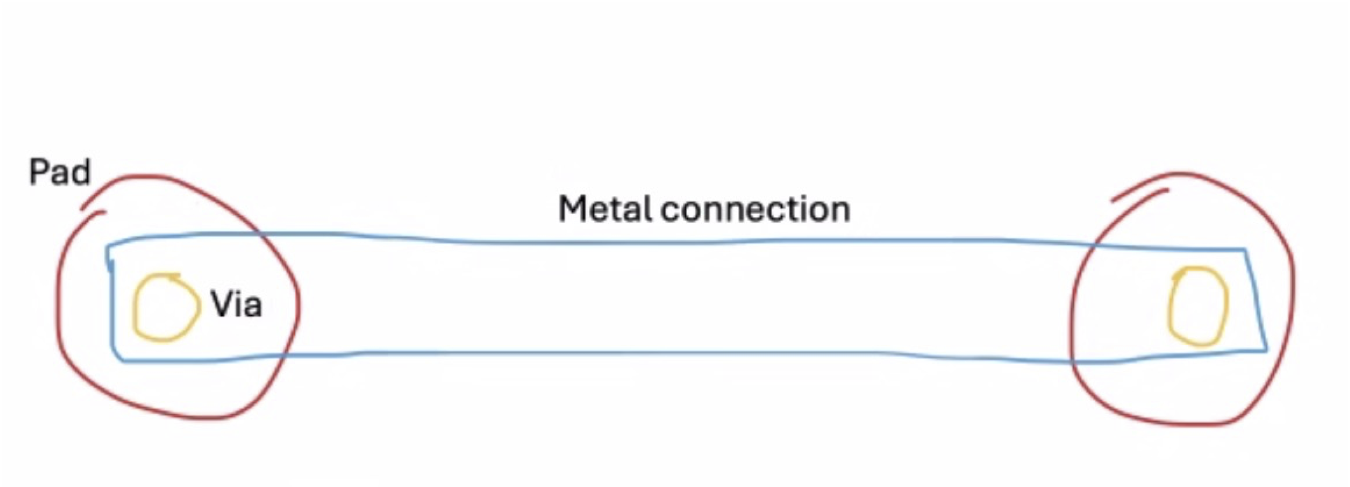
\includegraphics[width=0.5\linewidth]{sketch.png}

\textbf{Prompt for Test 6:}"I have sketched a design for 3d packaging, where we have a metal connecting two TSVs , please generate the python code to draw a GDSII based on the sketch. each color represents an individual layer. The metal connection should fully cover the vias, extending slightly beyond their edges. Ensure the metal connection is slightly wider than the via diameter to provide full coverage."; with graphical input of the sketch: 

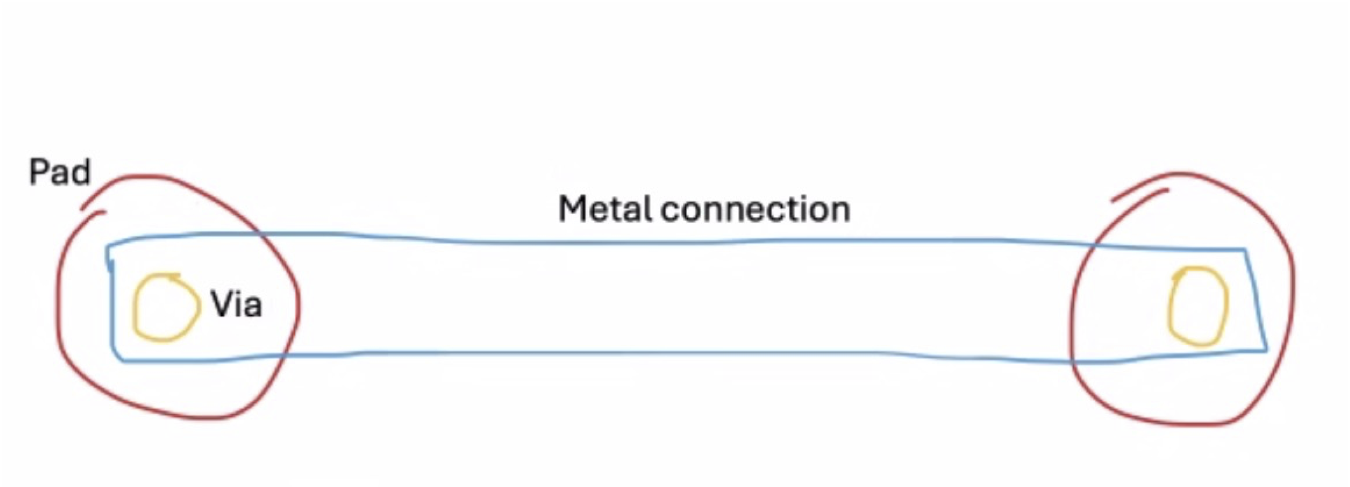
\includegraphics[width=0.5\linewidth]{sketch.png}


\begin{figure}[!h]
\centering
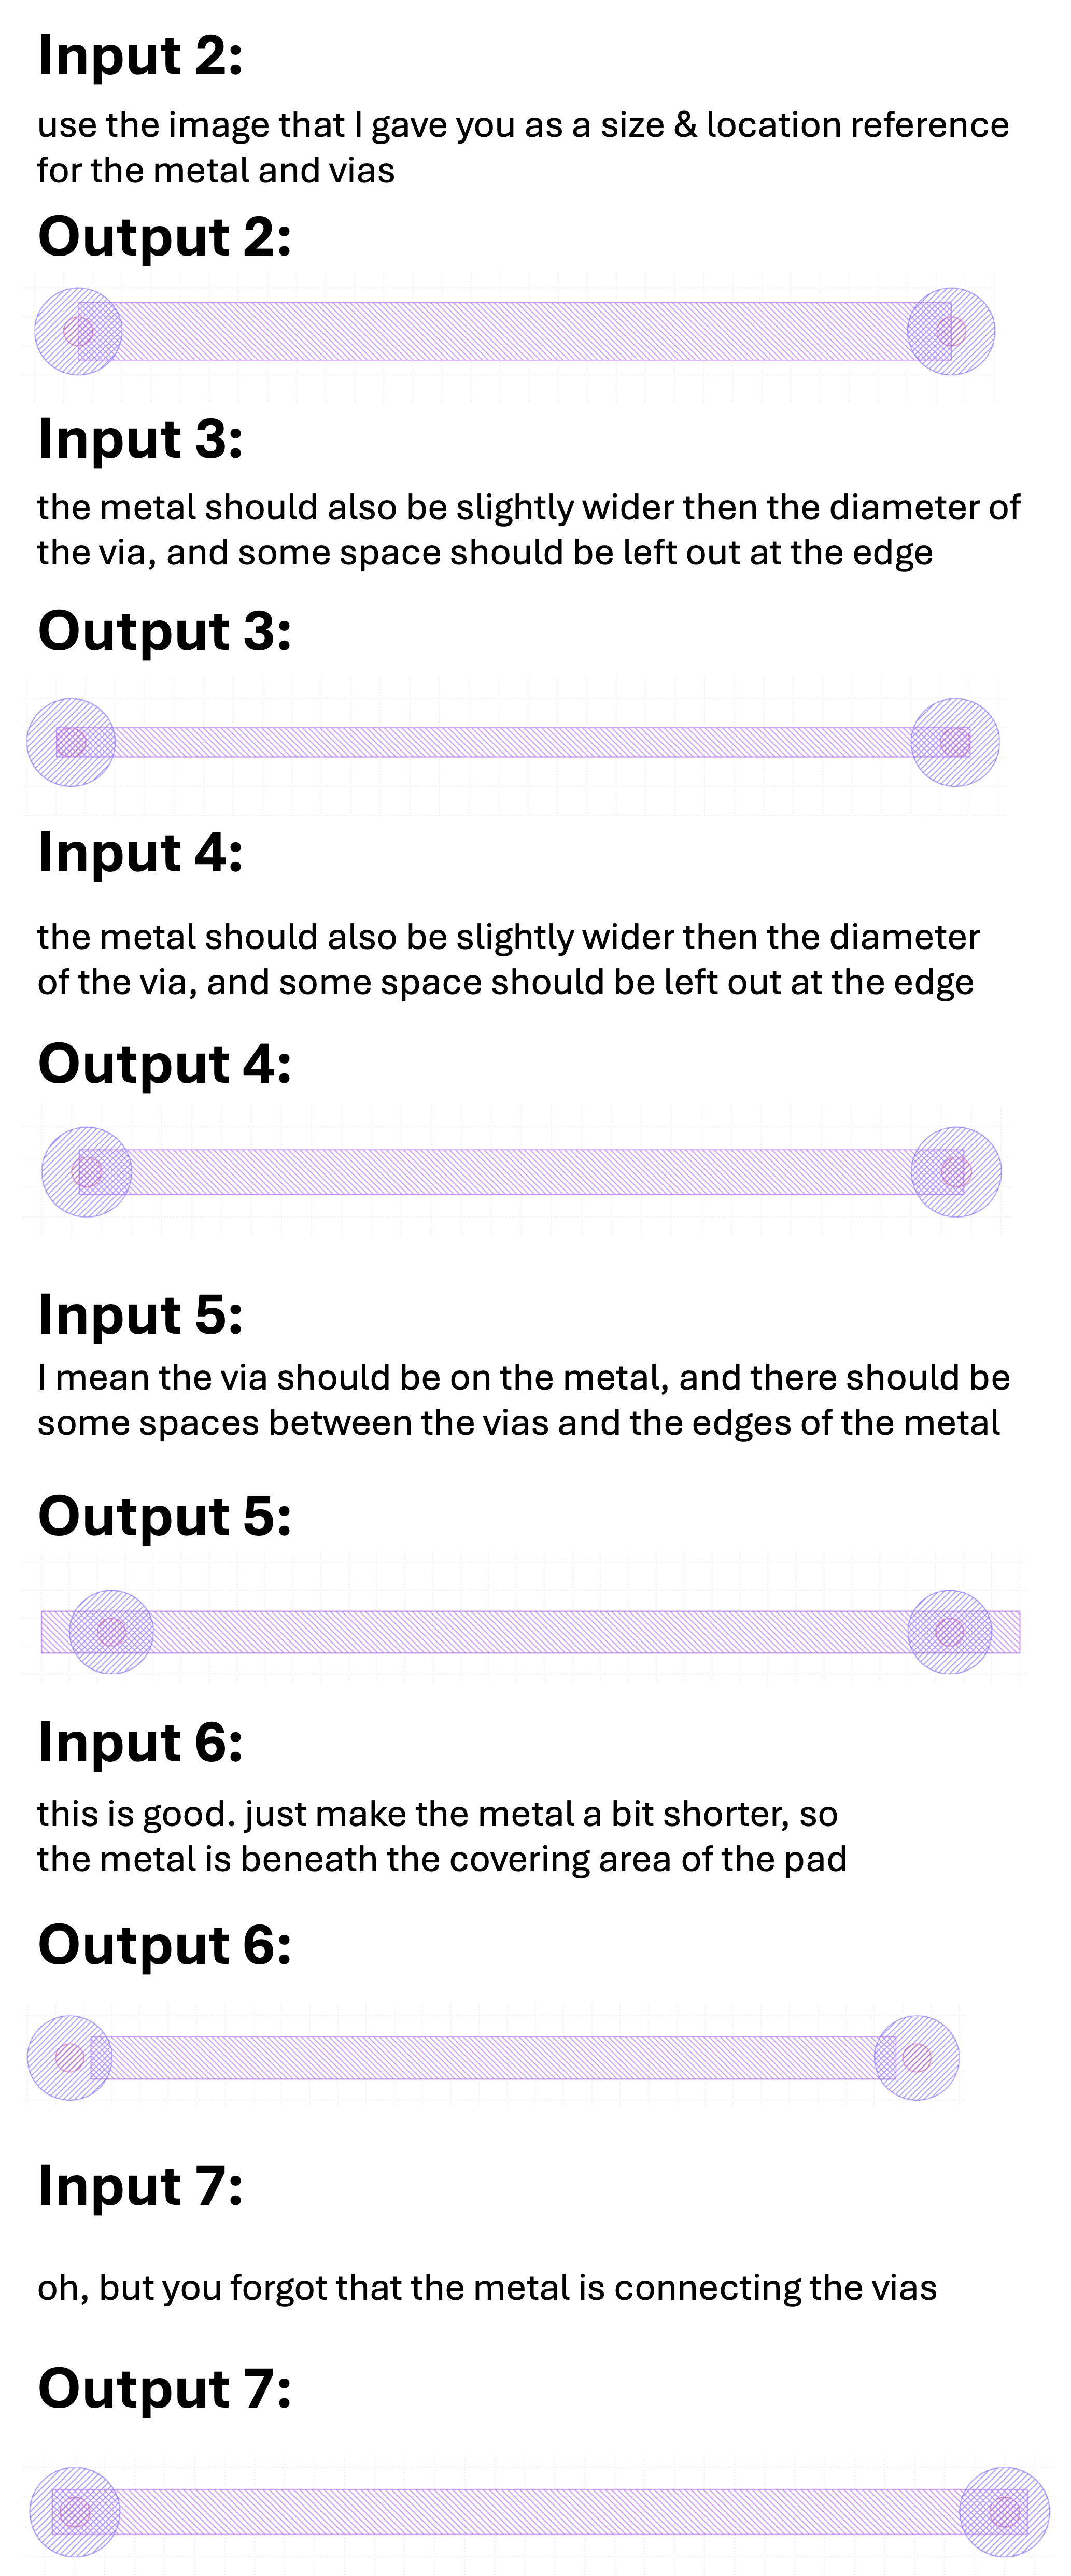
\includegraphics[width=0.5\linewidth]{Styles/Test3.png}
\caption{Test 3 - Iterations to guide the model to generate desired output}
\label{fig:test3_chat}
\end{figure}

\end{document}